\documentclass{sigchi}

% Copyright
\CopyrightYear{2020}

\toappear{
    Permission to make digital or hard copies of part or all of this work for personal or classroom use is granted without fee provided that copies are not made or distributed for profit or commercial advantage and that copies bear this notice and the full citation on the first page. Copyrights for third-party components of this work must be honoured. For all other uses, contact the owner\hspace*{.5pt}/author(s). \par\smallskip
    \copyright\ \the\copyrtyr\ \plainauthor
}

% Arabic page numbers for submission.  Remove this line to eliminate
% page numbers for the camera ready copy
\pagenumbering{arabic}

% Load basic packages
\usepackage{balance}       % to better equalize the last page
\usepackage{graphics}      % for EPS, load graphicx instead 
\usepackage[T1]{fontenc}   % for umlauts and other diaeresis
\usepackage{txfonts}
\usepackage{mathptmx}
\usepackage[pdflang={en-GB},pdftex]{hyperref}
\usepackage{color}
\usepackage{booktabs}
\usepackage{textcomp}

% Some optional stuff you might like/need.
\usepackage{microtype}        % Improved Tracking and Kerning
% \usepackage[all]{hypcap}    % Fixes bug in hyperref caption linking
\usepackage{ccicons}          % Cite your images correctly!
% \usepackage[utf8]{inputenc} % for a UTF8 editor only


% Paper metadata (use plain text, for PDF inclusion and later
% re-using, if desired).  Use \emtpyauthor when submitting for review
% so you remain anonymous.
\def\plaintitle{Automation of ordering processes in the industry 4.0}
\def\plainsubtitle{Developing a Prototype for a Service Button with Authentication Abilities}
\def\plainauthor{Finn Nils Gedrath, Leonard Pelzer}
\def\emptyauthor{}
\def\plainkeywords{industry 4.0, automation of ordering processes, internet of things, radio-frequency identification, amazon web services}
\def\plaingeneralterms{Prototyping, Seminar}

% llt: Define a global style for URLs, rather that the default one
\makeatletter
\def\url@leostyle{%
  \@ifundefined{selectfont}{
    \def\UrlFont{\sf}
  }{
    \def\UrlFont{\small\bf\ttfamily}
  }}
\makeatother
\urlstyle{leo}

% To make various LaTeX processors do the right thing with page size.
\def\pprw{8.5in}
\def\pprh{11in}
\special{papersize=\pprw,\pprh}
\setlength{\paperwidth}{\pprw}
\setlength{\paperheight}{\pprh}
\setlength{\pdfpagewidth}{\pprw}
\setlength{\pdfpageheight}{\pprh}

% Make sure hyperref comes last of your loaded packages, to give it a
% fighting chance of not being over-written, since its job is to
% redefine many LaTeX commands.
\definecolor{linkColor}{RGB}{6,125,233}
\hypersetup{%
  pdftitle={\plaintitle: \plainsubtitle},
% Use \plainauthor for final version.
  pdfauthor={\plainauthor},
  %pdfauthor={\emptyauthor},
  pdfkeywords={\plainkeywords},
  pdfdisplaydoctitle=true, % For Accessibility
  bookmarksnumbered,
  pdfstartview={FitH},
  %colorlinks,
  citecolor=black,
  filecolor=black,
  linkcolor=black,
  urlcolor=linkColor,
  breaklinks=true,
  hypertexnames=false
}

\newtheorem{principle}{Principle}[section]

% create a shortcut to typeset table headings
\newcommand\tabhead[1]{\textit{#1}}

% End of preamble. Here it comes the document.
\begin{document}

\title{\plaintitle}
\subtitle{\plainsubtitle}

\numberofauthors{2}
\author{%
  \alignauthor{\\Finn Nils Gedrath\\
    \affaddr{TH Köln}\\
    \affaddr{Gummersbach, Germany}\\
    \email{finn\_nils.gedrath@smail.th-koeln.de}}\\
  \alignauthor{\\Leonard Pelzer\\
    \affaddr{TH Köln}\\
    \affaddr{Gummersbach, Germany}\\
    \email{leonard.pelzer@smail.th-koeln.de}}\\
}


\teaser{
    \center
    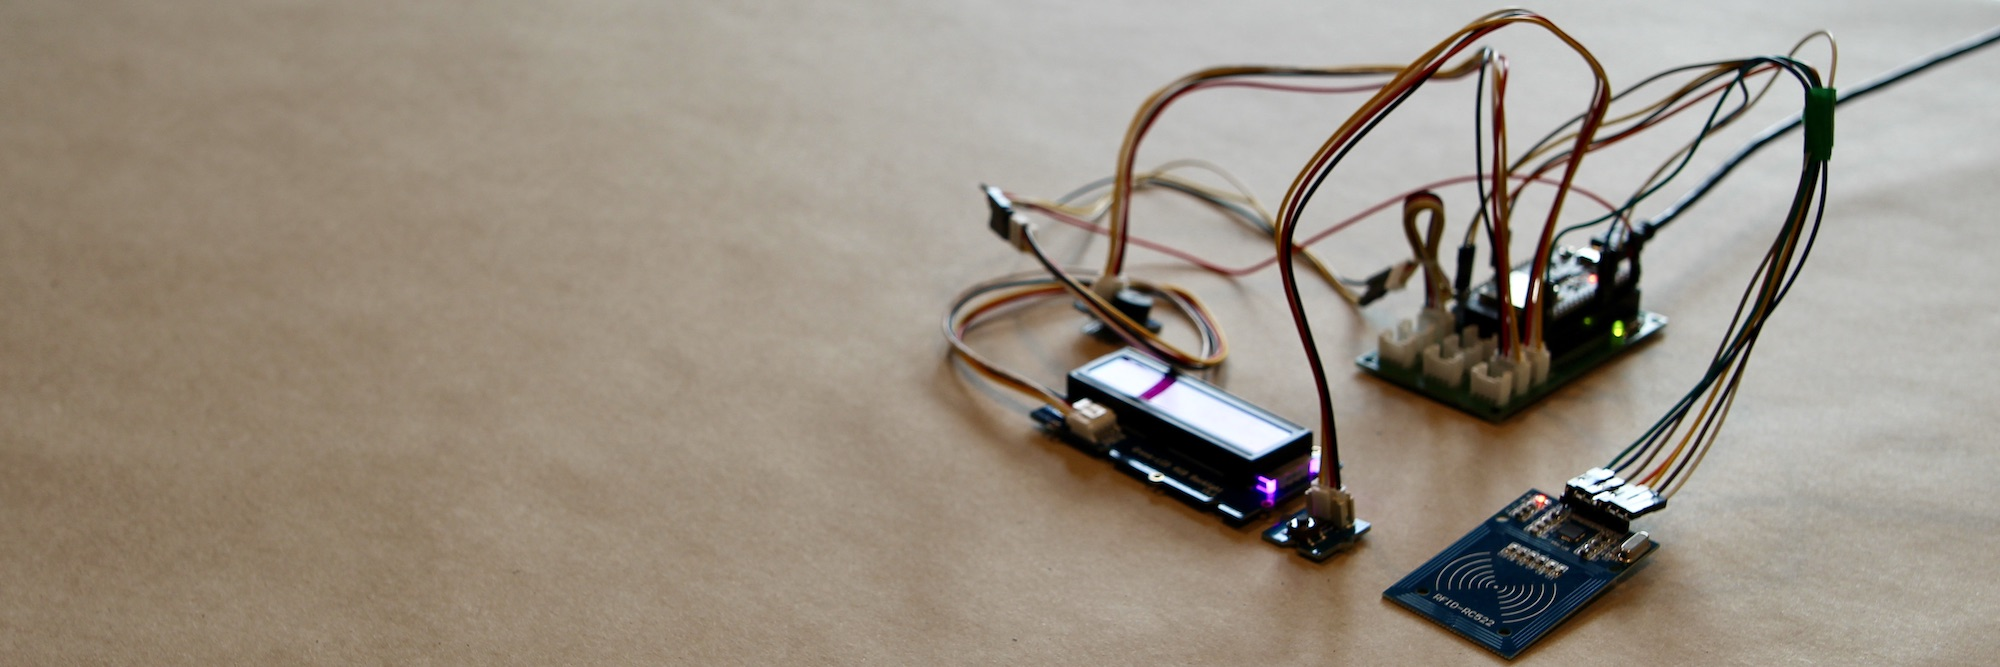
\includegraphics[width=\textwidth]{figures/microcontroller.jpeg}
    \caption{Finished prototype of a service button using ESP32 and Grove sensors and actuators.}
}

\maketitle

\begin{abstract}
    The digitalization process is as prominent in modern industry 4.0 as in our day-to-day life. Our approach to such transformation is a service button that can help employees in various different contexts to reorder products or building blocks and is also setup with a authentication abilities. This product lives in the context of the internet of things and can be connected with different suppliers and other working processes. This term paper will focus on the conception and development of a prototype for a service button. It will highlight the context of use by examine the problem space and taking a closer look at the interaction with the system especially how an extra authentication step can be included in the process. We will also discuss the choices of used sensors, actuators and authentication procedures and the paradigms of system architecture. We will conclude by discussing various ethics and security parameters and by taking a look at possible transformations to a ready-to-use product.
\end{abstract}


% ACM Classfication
\begin{CCSXML}
<ccs2012>
    <concept>
        <concept_id>10003120.10003138</concept_id>
        <concept_desc>Human-centered computing~Ubiquitous and mobile computing</concept_desc>
        <concept_significance>500</concept_significance>
    </concept>
    <concept>
        <concept_id>10010520.10010553</concept_id>
        <concept_desc>Computer systems organization~Embedded and cyber-physical systems</concept_desc>
        <concept_significance>300</concept_significance>
    </concept>
</ccs2012>
\end{CCSXML}

\ccsdesc[500]{Human-centered computing~Ubiquitous and mobile computing}
\ccsdesc[300]{Computer systems organization~Embedded and cyber-physical systems}

% Author Keywords
\keywords{\plainkeywords}

% Print the classficiation codes
\printccsdesc



\section{Introduction}
\label{sec:Intro}

The following term paper was developed as part of the course \textit{Internet of Things} taught by Prof. Dr. Matthias Böhmer in the advanced module \textit{web development} in the study course of media informatics at the TH Köln.

The central task was to concept and create an operable prototype in the Internet of Things (IoT) using different sensors and actuators while also communicating with different remote devices, which can suggest solutions for certain problems in a given context of use. The topic of this project is the development of a prototype of a Service Button in an industrial context, which gives an employee the ability to order any kind of stock at the point where he or she needs it. The Proposal for this project has been made by the \textit{Open IoT Lab Deutsche Telekom}\footnote{\url{https://iot.telekom.com/de/telekom-open-iot-labs}}.

\section{Problem Space}
\label{sec:Problem-Space}

Digitalization plays a major role in all areas of our lives today. Many processes are automated to the extent that they will function without human intervention. In today's industry, the automation of processes has the highest priority.
One of the key developments is the move towards \textit{Industry 4.0}, where individual production machines communicate with each other and consumables are automatically reordered \cite{Wollschlaeger:IoTIndustry4.0:2017}.
However, there are still many fields and use cases where manual intervention by a human is necessary. A Service Button can offer a way to automate and accelerate such use cases, where products need to be reordered from different suppliers.

These Service Buttons can be used in a variety of industrial contexts. Some of them could be vehicle production sites where important assembly parts have to be reordered, chemical laboratories where chemicals and equipment is used up in a short period of time or hospitals where medical equipment needs to be in stock at all times. All these contexts have different safety and security regulations. Nevertheless, it es very important that a Service Button is adaptable to any given context since its purpose is to support and fasten current working processes.

Each Service Button needs to be allocated in close proximity to a stocking place for a specific item. One Service Button is directly assigned to a product. Through interacting with a Service Button an order with a fixed number of items is placed and send to either the supplier directly or control unit which can be a manager or a different employee.

\paragraph{Existing Products: Amazon's Dash button}

There are some existing products on the market which try to solve similar problems. One approach is \textit{Amazon's Dash button}. It gave the customer the possibility to order a product from Amazon at the push of a button. The product range was limited to typical household consumer products. 

Concerns were raised among others by a german ruling stating a violation to consumer protection law. Neither a price nor enough information to the success of an order were accessible since there was no display on the device. Amazon developed protection features by sending a notification message to the users phone when an order is placed. The Amazon's Dash buttons were discontinued by Amazon at the end of 2019 and replaced by virtual Dash buttons. \cite{Online:TheVerge:DashbuttonCourt, Online:TheVerge:DashbuttonDiscontinued}

It is still questionable whether a virtual version of a dash button can trigger a similar user experience that was intended for the physical Dash button. Originally the interaction would take place in the physical space at the moment when the need for a specific product arises.

\paragraph{User Needs and Requirements}

In the following a smaller group of stakeholders are determined: \textit{Employee}, \textit{Department Manager}, \textit{General Manager}, \textit{Supplier}. The employee is the only stakeholder that will interact with the system directly, making that group the primary stakeholder. The managers and suppliers are specified as secondary stakeholders as they will interact with the system only in some rare use cases.

From an employee's point of view the most important need is the ease of use. Interacting with the Service Button must be faster than traditional working processes. Therefore a Service Button needs to be placed in close proximity to the users working station or stocking place. The system must also highly conform to the principals of \textit{self-descriptiveness} and \textit{learnability} \cite{ISO:9241-110:2020}. On the other hand the system must be \textit{efficient} \cite{ISO:9241-110:2020} to use, especially for users who have interacted with the system many times before. For an employee it should be possible to cancel an incorrect order if they started a transaction unintentionally or interacted with the wrong Service Button which means that the system should also be \textit{robust against user errors} \cite{ISO:9241-110:2020}.
Finally the user must be able to see the state of the system throughout the interaction, especially at the end where whether the transaction has been successful or not.

From the department managers or general managers point of view, it should be traceable at which time and by which employee the products were ordered, to have an overview of the whole ordering and supply system and to regulate orders if needed. Furthermore, these stakeholders may want to restrict usage abilities of the Service Button, so that an employee can only use the Service Buttons from his or her department.

There are also technical requirements. The Service Buttons need a power supply, which should be very flexible due to the positioning in the production halls. Access to a network is also necessary to enable the successful sending of an order.

\section{Human Interaction with the System}
\label{sec:Interaction}

Since the Service Button gives the user the ability to start an interaction in the whole sociotechnical system especially the order process, it is crucial to take a closer look at how this interaction is designed and what user experience is intended through that design.

\begin{figure*}
    \center
    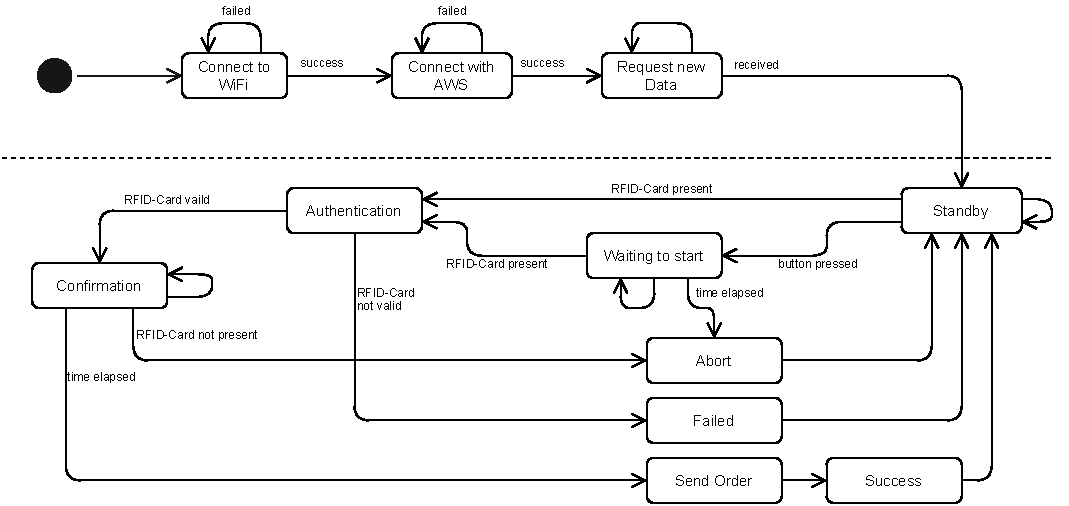
\includegraphics[width=\linewidth]{figures/states.drawio.pdf}
    \caption{Representation of states throughout the setup phase (1 – 3) and the Interaction in the order process.}
    \label{fig:states}
\end{figure*}

As discussed in chapter \ref{sec:Problem-Space} one requirement is to control every transaction with a verification step, to prevent an unauthorised user from interacting with the system. This is done completely using the Service Button and not on any other device such as a smartphone, thus ensuring that the interaction is efficient and has no unnecessary interaction step. In addition, depending on the domain, smartphones are not allowed due to security regulations. Only after a successful authorisation can an order be placed (see Figure \ref{fig:states}). This is implemented with an RFID transponder, as this is already used in many domains to unlock doors and specially protected areas. A detailed discussion of this is given in chapter \ref{sec:Technologies:Sensors-Actuators}. Other authorisation types are also imaginable.

\paragraph{Starting the Interaction}
Let us assume the user of the system wants to send an order because he or she is short of a specific item and wants to do that with the micro-controller. The only step that is mandatory for the transaction is the authorisation. If the user holds the RFID transponder to the micro-controller, the authorisation can start and the order can be completed.

The only problem with that is that the user can't be sure how to start the transaction the first time he or she uses it. From the perspective of the cognitive sciences, Norman distinguishes between \textit{affordances} and \textit{signifier} for interaction elements \cite{Norman:EverydayThings:2013} especially in a physical space. Although the system has the affordance that a transponder can be held to the RFID sensor, it lacks the corresponding signifier that makes it clear to the user how to interact with it. We argue that a button is a larger signifier because we are very much trained to click on a button. A specific product design can help to make it clear to the user how to start a transaction (see chapter \ref{sec:Future}).

However, it is important to give the user the possibility to take only the important steps in his or her interaction. Especially users who have been familiar with the system for a long time might be frustrated by this unnecessary step. On the other hand, starting the interaction via the button must still be possible as discussed earlier in order to be robust against \textit{user errors}, as standardised by the ISO 9241-110:

\begin{principle}{User error robustness.}
The interactive system assists the user in avoiding errors and in case of identifiable errors treats them tolerantly and assists the user when recovering from errors. \cite{ISO:9241-110:2020}
\label{prin:UserErrorRobustness}
\end{principle}

Thus, there should be a button as well as the presentation to the RFID sensor as an entry point into the interaction. Figure \ref{fig:states} shows this possibility in detail.

\paragraph{Confirmation of a transaction}

Another point that emerges from the principal of \textit{user error robustness} is that the user should be given the opportunity to undo an unwanted action or that the system should ask for confirmation. Thus, as described in Figure \ref{fig:states}, the system should provide a time frame in which she can cancel the transaction. During the development of the prototypes there were different iterative approaches:

In the first option, the user is asked to click the button if she wanted to cancel the transaction. When he or she is sure he or she wants to complete the transaction, the user would have to simply wait and ignore the text. The problem that occurred especially through some small testing is that the user was asked to do something that he or she should ignore in a positive scenario (the positive scenario is the intended order). So there is a conflict between the system's request and the user's aim to fulfil the user's task. Furthermore, in a negative scenario, where the user wants to cancel the transaction, the active click of a button may be too slow. To do this, the user must first remove the RFID chip from the sensor and try to hit the button with his or her finger. This can be difficult for users with cognitive or physical disabilities or in stressed working environments.

Therefore, a version was developed that allows the user to abort a transaction. This version uses the \textit{undo} interaction style, which can be found mainly in word processing programs or in the web browser. Here, pressing a button or a key combination \texttt{CMD+Z} / \texttt{CTRL+Z} retrieves the last change. This interaction style can also be applied to this use case. As described above the transaction can be started by holding the RFID sensor in front of micro-controller. If the employee wants to undo the start of this transaction, he or she can do so by undoing his or her physical action by simply removing the transponder.

In addition, the system must always provide feedback on when it is okay to remove the transponder, so that the user does not remove the transponder from the micro-controller too early due to unawareness.

\paragraph{System Response throughout the Interaction}

For the user it is very important that the system informs the user in which state she is currently, as standardised by ISO 9241-110:

\begin{principle}{Self-descriptiveness.}
The interactive system presents appropriate information, where needed by the user, to make its capabilities and use immediately obvious to the user without the need for unnecessary user-system interactions. \cite{ISO:9241-110:2020}
\end{principle}

In theory it is possible to give the user feedback through optical, auditory or tactile signals. We decided to use optical and auditory signals as the user is not likely to touch the Service Button in the interaction. The display is used to display the current state of the system. One challenge with displaying text on a small display is that the available space is limited to a defined number of characters. Due to that the message must be as short as possible while still being precise and giving the user enough information during the interacting on what she needs to do next. A full list of messages presented to the user can be seen in Table \ref{tab:display-outputs}.

The buzzer will give off different auditory signals according to the status of a response being either successful, fallacious or pending. This is done by having different lengths and repetitions of signals: A long signal supports error messages where a shorter signal supports a success message. Shorter signals with a repetition are used to indicate the response of the system is still pending.

\begin{table}
    \center
    \begin{tabular}{l l}
        \tabhead{System-State} & \tabhead{Display-Text}\\
        \midrule
        Connect to WiFi & \texttt{Try connecting to WiFi} \\
        Connect with AWS & \texttt{Try connecting to AWS} \\
        Request new Data & \texttt{Setting up...} \\
        \midrule
        Standby & \texttt{[PRODUCT]} \\
        Waiting to start & \texttt{Hold RFID-Card to Sensor} \\
        Authentication & \texttt{Checking...} \\
        Confirmation & \texttt{[PRODUCT] Menge: [N]x} \\
        \midrule
        Abort & \texttt{Abort Process} \\
        Failed & \texttt{Not Autherized} \\
        Send Order; Success & \texttt{Success} \\
    \end{tabular}
    \par\smallskip
    \caption{Display outputs in a specific state of the system (see Figure \ref{fig:states}). Text displayed in brackets are placeholders since the micro-controller is to be configured to a specific product.}
    \label{tab:display-outputs}
\end{table}


\section{Choice of technologies}
\label{sec:Technologies}

On the knowledge gained from the previous chapters, we decided on the technologies we wanted to use. The expert lectures from the module served as a basis for this. 
We decided to use RFID technology in order to offer an added value compared to conventional Service Buttons. Furthermore, we used the MQTT protocol for the communication with the backend.

\subsection{Sensors and Actuators}
\label{sec:Technologies:Sensors-Actuators}

Sensors and actuators are crucial in developing products and prototypes in the internet of things. They help to measure properties of the world so that users can interact with a system and they can change properties of the world thus communicating to the user \cite{ISO:20924:2018}.

In the prototype we used two sensors and two actuators. As sensors we used a RFID reader and a button. With the help of a RFID senor it is possible to read the data from a RFID card. This works with the help of induction. The reader generates a electromagnetic field that induces a voltage in the RFID card. The RFID card then influences the electromagnetic field of the reader and transmits the data. \cite{Adryan:TechFound-Components:2017}

In many companies, employees have access cards for different areas. In most cases, these access cards are also RFID cards. We want to use these cards as an authentication option for the service buttons. The RFID reader is the central element of interaction. It can be used to start and stop the interaction. The button serves as a second interaction option.

Fingerprint sensors or face scanners could also be used as alternative authentication options. The advantage over RFID cards would be that the employees do not need a card and could not use cards from other employees. However, these authentication options would be more complex to implement. Each employee would have to scan the biometric data once personally. An RFID card can simply be handed over to them. 

As actuators we used a buzzer and a display. They give the user feedback on the ordering process. The buzzer can make a beeping sound. The display has rgb and blacklight and communicates with the ESP32 via an I2C interface.

\begin{figure}
    \center
    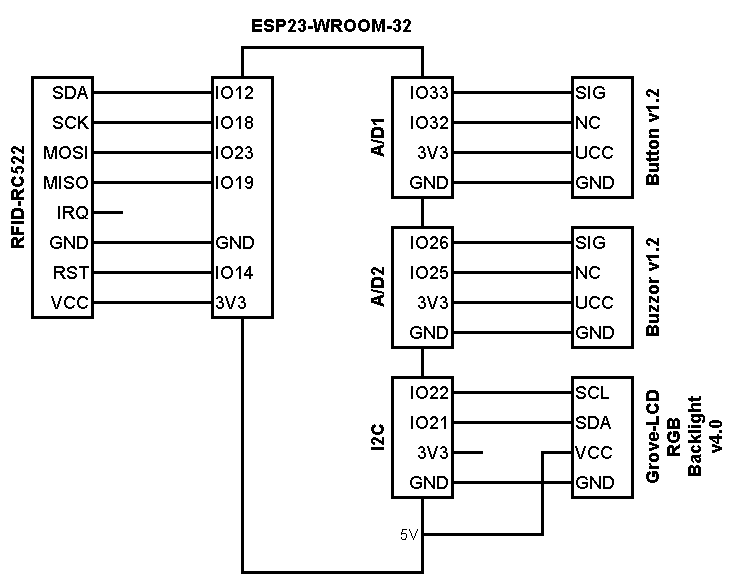
\includegraphics[width=\linewidth]{figures/schematics.drawio.pdf}
    \caption{Schematic representation of the connections of sensors and actuators with ESP32.}
    \label{fig:schematics}
\end{figure}

We connected the buzzer and the button using \textit{Grove Universal 4 Pin} cables. The challenge with the display was that the intended connector on the ESP-32 could not supply a 5V voltage. So we had to take the Grove Universal cable apart and connect a partial cable to a 5V connector. We connected the RFID reader using jumper cables. A graphic demonstrating which connectors we used is shown in Figure \ref{fig:schematics}.


\subsection{System Architecture}
\label{sec:Technologies:Architecture}

Having a Service Button alone is not enough to give the user the ability to place an order. The System needs a functioning infrastructure to send the order from the micro-controller to a supplier or a different unit in its organisation. The communication between different components of a distributed system can be realised either as a synchronous or asynchronous pattern. Using an asynchronous pattern like publish/subscribe has the strong advantage of decoupling the senders and receivers messages that are sent in the system. This can prevent the loss of messages in cases of temporary unavailability which is a common problem in a distributed system. Furthermore, the publish/subscribe pattern gives the ability to send messages to many receivers at once by using topics that a receiver can subscribe itself to. \cite{Adryan:TechFound-Network:2017}

There are many open protocols that can be used to accomplish an asynchronous communication system. Besides \textit{AMQP} and \textit{XMPP} we have chosen \textit{Message Queue Telemetry Transport (MQTT)} \cite{ISO:20922:2016} because of its ease of operation. The messages sent between the components are very small and the protocol enables a lossless communication over lossy networks \cite{Adryan:TechFound-Network:2017}. MQTT-Messages are send on top of TCP/IP in the Application Layer. All messages are sent to a central \textit{MQTT-Broker} which then reroutes the messages by having the connected components subscribed to a specific topic. In our prototype we used the \textit{Amazon Web Services (AWS)} as our MQTT-Broker (see Section \ref{sec:Backend}).

The MQTT-Protocol also has the advantage that all messages can have several configuration options on how high the assurance level for a delivery of a message. As standardised by the ISO/IEC \cite{ISO:20922:2016} there are three different types of \textit{Quality of Services (Qos)}: Types 0, 1 and 2. By sending a message with the QoS-Flag set to 0 (at-most-once), the sender has no guarantee that the message has been received by the addressee since he will not send a confirmation message. This is very resource friendly and is applicable to data that is not required to get to its receiver because, for example, it might be weather data that is sent in a short period of time anyway. In levels 1 (at-least-once) and 2 (exactly-once) extra acknowledgement messages are sent between receiver and sender. Level 2 also guarantee that the message will only be received once and no more.

It is clear that it is important to assume that messages sent between the components should not to get lost. Therefore messages sent in the prototype should have the QoS-Flag set to either 1 or 2. A more detailed discussion of that is given in Chapter \ref{sec:Backend:Messages}.

We have discussed the paradigm used for the communication between the micro-controller and the central administration instance. Now we want to take a look at how the micro-controller can communicate in this instance on a technical level.

It is clear to say that the Service Button has to have access to the local network. We have decided to take a simple approach to creating the prototype: The micro-controller establishes a direct connection to the local WiFi network and communicates via the router with the Internet and the administration instance using IP-based protocols. This setup can be seen in Figure \ref{fig:architecture} where every micro-controller (ESP32) has a direct connection to the MQTT-Broker.

\begin{figure}
    \center
    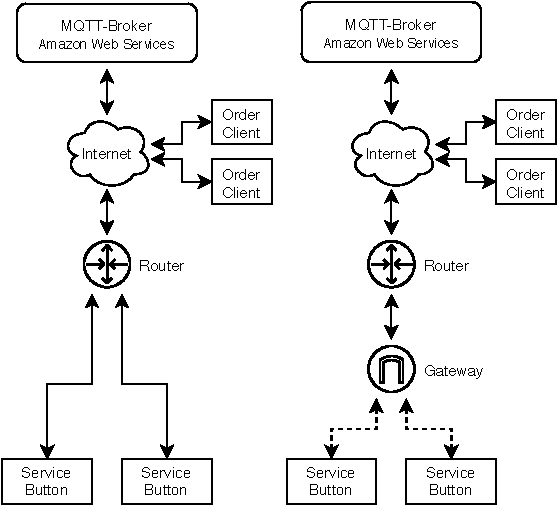
\includegraphics[width=\linewidth]{figures/architektur.drawio.pdf}
    
    \caption{The micro-controllers are either connected to the internet over IP-based protocols (left) or non-IP-based protocols over an extra Gateway (right). The MQTT-Broker services as an asynchronous communication tool between the micro-controllers and the other clients and can be addressed over the internet.}
    \label{fig:architecture}
\end{figure}

Using this setup has the advantage that testing in development is simplified to the degree of having just one component that needs testing. The Experience a user has with this system is the same as in any other setup, thereby the system qualifies as a liable proof-of-concept. But there are many disadvantages of using such setup in a production environment. For example, the micro-controller consumes a lot of power establishing an IP based connection to the Internet. In a scenario where the Service Buttons have to be located at any given space even if a consistent power supply is questionable. Furthermore having each controller responsible for the WiFi connection can be a difficult task to setup and maintain because \texttt{SSID} and password have to be inserted for each device. In addition it is questionable that a WiFi connection can be supported in many domains because of security reasons.

A solution to the problems mentioned above can be the use of a \textit{Dedicated Local Gateway}, which establishes a communication path between the Service Button and the network router (see Figure \ref{fig:architecture}). This makes it possible to use non-IP based protocols between the gateway and the Service Button. Examples of such non-IP based protocols are ZigBee, LoRa and LPWAN. These protocols require much less energy to send and therefore have less impact on the general power budget. Since now only the gateway communicates over IP-based protocols with the network router, only the gateway needs to know the WiFi network parameters allowing for easier maintenance. In order to connect Service Buttons in larger areas via such alternative protocols, the corresponding routers or beacons can be used, depending on the choice of protocol. \cite{Adryan:TechFound-Components:2017}

\section{Implementation of the IoT-Backend}
\label{sec:Backend}

The central task of the Backend as discussed in Chapter \ref{sec:Technologies:Architecture} is to enable a connection between each part and to move as much processing-overhead as possible away from the Service Button to sustain power. In the following we want to discuss how we have implemented these communication channels.

Since we decided to use the MQTT-Protocol we made use of the Amazon Web Services (AWS) which offers Platform-as-a-Service cloud computing in our prototype. AWS is a subsidiary of the company Amazon and its business model is to provide cloud computing for other companies \cite{Online:Amazon:AWS}. 

The use of AWS offers many advantages: Firstly, the setup with AWS can be very easy since there are many pre-configured solutions out there. AWS can also be configured to react to a specific event by making use of the AWS Lambda Functions. Companies therefore do not need their own cloud computing providers and the pricing can be configured to be dependend on the actual use. Additionally to this, AWS is characterised by its high stability. By making use of the \textit{sharding pattern} there are different, global distributed data centres which can take over the tasks of other data centres in case of a failure like power shortages or physical damage  \cite{Online:Amazon:AWSFAQ}. Not only that, AWS enables \textit{horizontal scalability} for the entire system. Thus, further computing capacities can be easily added as the number of Service Buttons increases and computing power is needed. However, it is still possible to implement the same or similar system with a different cloud service, or even a local server. There are many Open Source Projects like HiveMQ\footnote{\url{https://www.hivemq.com/}} or Mosquitto\footnote{\url{https://mosquitto.org/}} that can be used for free. 

\subsection{Sent messages between the components}
\label{sec:Backend:Messages}

\begin{table*}
    \center
    \begin{tabular}{lclll}
        \tabhead{Topic-Name} & \tabhead{QoS} & \tabhead{Structure of the Payload} & \tabhead{Comment} \\
        \midrule
        \texttt{setup/\{5\}} & \texttt{1} & \texttt{\{1\};\{2\}} & Change of product name and quantity order. \\
        \texttt{auth/\{5\}} & \texttt{1} & \texttt{\{3\};\{4\}} & New RFID chip to one or all dash buttons. Chaining possible. \\
        \midrule
        \texttt{order} & \texttt{2} & \texttt{\{1\};\{2\};\{5\};\{4\}} & Submit a new order. \\
        \texttt{init} & \texttt{1} & \texttt{\{5\}} & The micro-controller (re-)started and needs Chip-IDs. \\
    \end{tabular}
    \par\smallskip
    \caption{ List of topics used to send MQTT-Messages between the micro-controller and other clients. These topcis are defined in the Dashboard of the Amazon Web Services (AWS). \textit{\texttt{\{1\}} = Product name. \texttt{\{2\}} = Order quantity. \texttt{\{3\}} = Operater (POST/DELETE). \texttt{\{4\}} = UID of RFID-Chip. \texttt{\{5\}} = UID of Service Button.}}
    \label{tab:mqtt-topics}
\end{table*}

As shown in Figure \ref{fig:states} the Prototype of the Service Button tries to connect to the configured local network and establishes a connection to the MQTT-Broker of AWS. After that the Service Button publishes an event to the \texttt{init} topic (see Table \ref{tab:mqtt-topics} for the Structure of the Payload). This event will then trigger an \textit{AWS Lambda Function}, a functionality to react to specific topics that are publish in the system, which will then automatically published the setup data stored at AWS to the \texttt{setup} topic. Now the Service Button has the necessary information such as the product name and quantity number to show to the user. Through the \texttt{init} event a list of Authentication Codes is sent to the Service Button which are used to authenticate the user over RFID. These are sent over the \texttt{auth} topic. The discussed QoS Flag for these messages is set to 1 (see Chapter \ref{sec:Technologies:Architecture}) since the messages can be received more than once because these messages, especially the \texttt{DELETE}-operator is idempotent.

All settings can also be changed during run-time over the \texttt{setup} and \texttt{auth} topics. Therefore it is possible to add another employee to the list of authorised personal or change the product or quantity that can be order from a single Service Button since one Micro-Controller can be addressed directly over the UID of the Service Button (see Table \ref{tab:mqtt-topics}).

After the \textit{Authentication} and \textit{Confirmation} steps are completed (see Figure \ref{fig:states}) the order is placed by raising an event to the \texttt{order} topic. This message is sent with the QoS-Flag set to 2 since multiple received messages would lead to multiple orders made by the company. However, having more parts/products in stock may not be that big of a problem. Therefore it can be argued if this flag can be set to 1 as well since using QoS 2 is storage and power consuming. The published order is now displayed in a AWS-Dashboard. In a real-world environment this can be easily extended to the fact that the order is automatically sent to a manufacturer.

\subsection{Backend Security}
\label{sec:Backend:Security}
The security of today's systems has become increasingly important in recent years. The integrity of stored data is not only a discussed topic in professional groups but also in todays society. It is therefore crucial to ensure the protection of data: therefore the Amazon Web Services (AWS) require the use of a Public Key/Private Key infrastructure that needs to be set up to enable the connection to AWS. The topics used in the system also have to be white-listed in the dashboard. This ensures that only the Service Buttons are allowed to publish MQTT messages to the corresponding topics. To take further precautions to ensure that no unauthorised messages are sent via the \texttt{order} topic, the UIDs of the ordering employee and a list of them on the server can be compared if the employee is authorised to place orders. 

To take that even further, the UIDs would not be stored on the Service Buttons but on the server. Since the waiting time in the interaction would be increase beacuse every UID has to be compared with the server first, until a corresponding reaction can be displayed on the Service Button, we decided to store the Data on the Service Button as well.

Although these precautions are taken, it can be said that no personal data is send over the system: Each employee is verified by his or her unique UID. This means that only randomly generated IDs, and no biometric data, are used for the entire verification process and are processed using the AWS. As a result, the data stored at AWS cannot be used to draw any conclusions about the person. Such inferences are only possible if there is a clear correlation between the UIDs and the names of the employees. This is only possible locally in the companies as they store these personal data.

\section{Discussion and Conclusions}
\label{sec:Future}

This term paper proposed a secure solution to a Service Button in an industrial context by enabling extra authentication steps. Through the developing process of our prototype we gained a few insights that may need to be considered in future developments of prototypes or a final product.

But there are some considerations that need to be taken into account. Since we made use of Amazon Web Services our proposed product has a big dependency on a large, globally active company over which small companies have no influence. Thus, the Service Buttons are ultimately dependent on Amazon's pricing policy. As already discussed in Chapter \ref{sec:Backend} the use of Amazon Web Service is not required since many alternatives exist. On the other hand, AWS offers many advantages, such as horizontal scalability and stability.

We also gained a few insights in terms of accessibility. When the prototype is transformed into a finished product, it is essential that it can also be used by people with cognitive or physical disabilities.
For example, the time span for cancelling the order must be taken into account. This is relatively short and requires quick action if you want to cancel the order process. This could be a problem for people with cognitive disabilities. Furthermore, the colouring of the display must be taken into account. Could this colouring represent a problem for people with visual impairments? Are the colour contrasts correct? It might also be important that the whole interaction is possible without having the ability to communicate without auditory or optical signals. To accomplish that, the buzzer that has been used in this prototype could be exchanged by RGB-Dioide to indicate the states of the system. Another idea would be to link specific individual settings to the UID of the RFID-card. Therefor, the colour contrasts of the display could be adjusted or the sounds of the buzzer could be changed according to the users settings. Since these requirements are outside the scope of this project they are not implemented in the prototype.

Another point that has come to our attention is the question of whether the RFID-card will not obscure the display. How big must the Service Button be to prevent this?

We conclude, that our prototype for a Service Button can find application in today's industrial contexts. It can automate the ordering processes and guarantee a smooth workflow. Especially in the context of Industry 4.0, Service Buttons offer a decisive advantage, because they allow consumables that cannot be tracked by machines to be easily re-ordered. 
The implementation of RFID technology offers a decisive complement to already known Service Button solutions. Furthermore, the Service Button is very flexible and can be configured specifically to the domain- and company-specific requirements due to the use of a flexible communication system and a display, as the configuration can easily be changed remotely.

\begin{figure}
    \center
    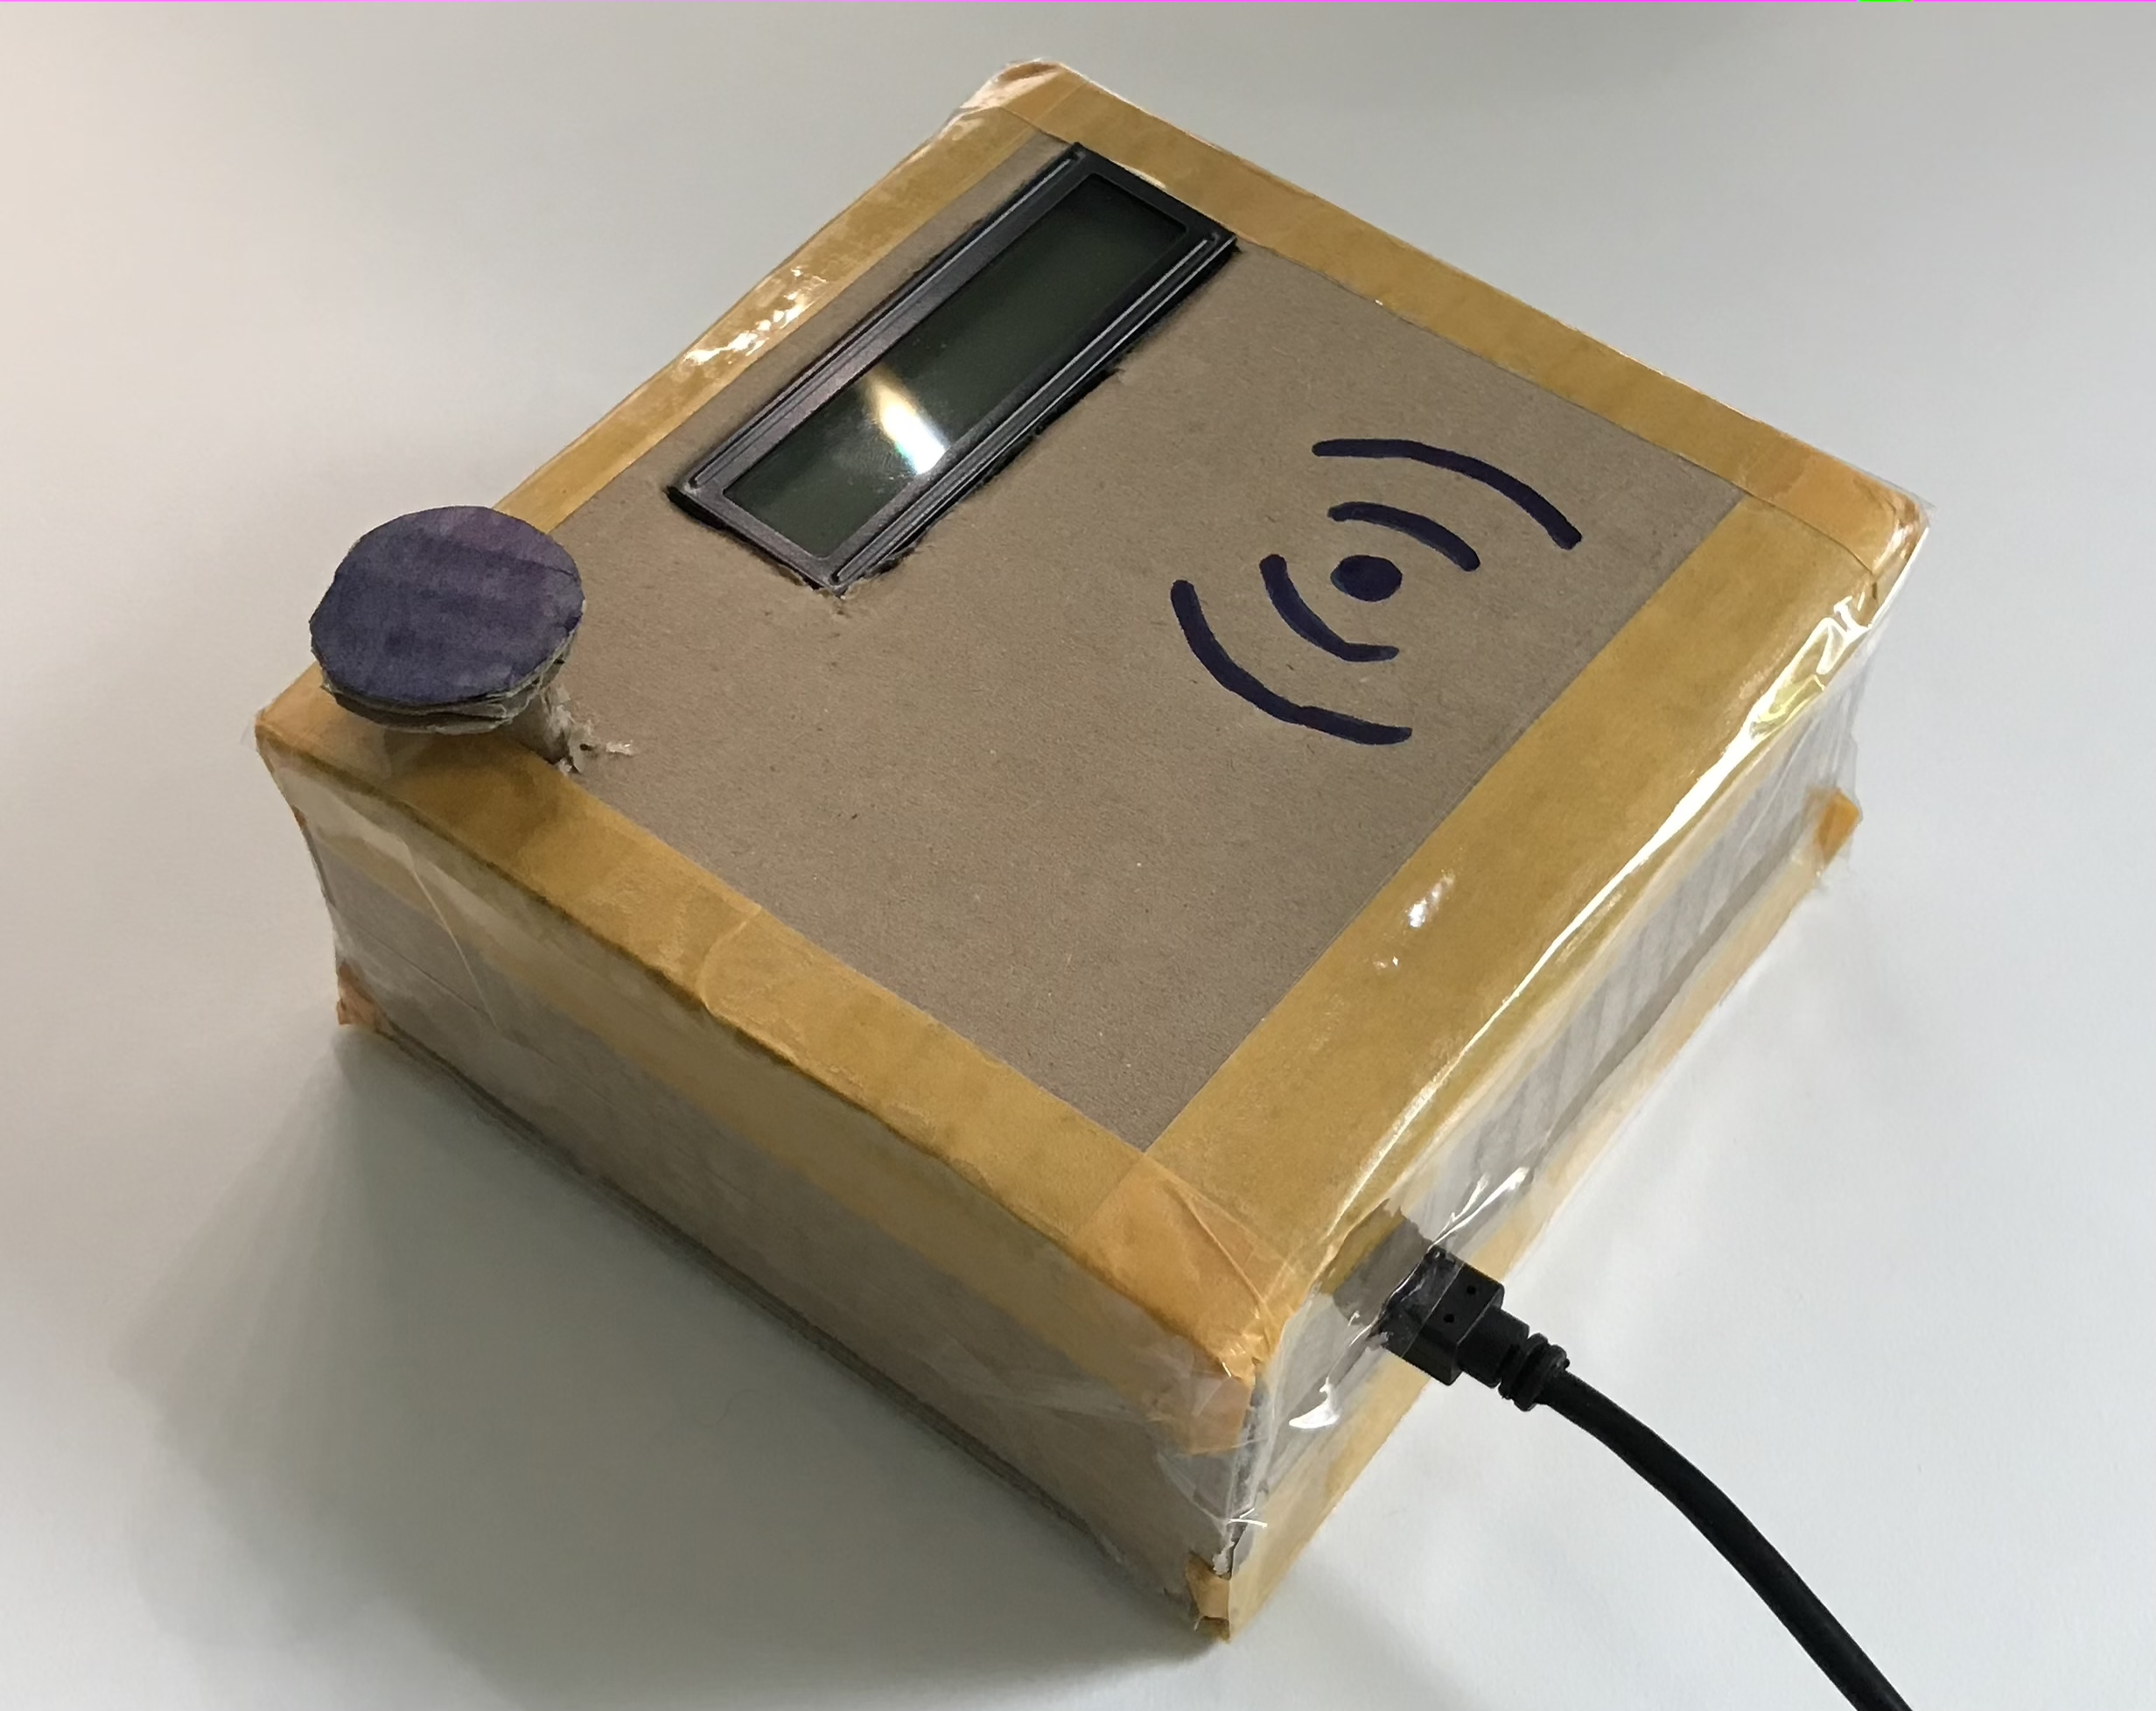
\includegraphics[width=\linewidth]{figures/prototype.jpg}
    \caption{To get a better feeling for the appearance of a finished product, we built a small housing for the prototype. As materials we used cardboard and adhesive tape. The RFID sensor can read the cards through the cardboard.}
    \label{fig:prototype}
\end{figure}


\balance{}

% REFERENCES FORMAT
% References must be the same font size as other body text.
\bibliographystyle{SIGCHI-Reference-Format}
\bibliography{literatur}

\appendix

\subsection{Open Source Project}

The entire development process is documented via Git on GitHub and is published as an open source project under the Apache 2.0 License.

\begin{itemize}
    \item Repository on GitHub: \\ \url{https://github.com/finnge/iot-service-button/}
    \item Website on GitHub Pages: \\ \url{https://finnge.github.io/iot-service-button/}
\end{itemize}

\subsection{Demo}

A video was made to see the prototype in use and to show its operability. It can be viewed under the following link: \\
\url{https://youtube.com/BLABLA}

\balance{}

\end{document}

%%% Local Variables:
%%% mode: latex
%%% TeX-master: t
%%% End:
